\documentclass[12pt]{article}
\usepackage{hyperref}
\usepackage{listings}
\usepackage[margin=1in]{geometry}
\usepackage{enumitem}
\usepackage{multicol}
\usepackage{array}
\usepackage{titlesec}
\usepackage{helvet}
\renewcommand{\familydefault}{\sfdefault}
\usepackage{amsmath}     % For math equations
\usepackage{amssymb}     % For advanced math symbols
\usepackage{amsfonts} % For math fonts
\usepackage{gvv}
\usepackage{esint}
\usepackage[utf8]{inputenc}
\usepackage{graphicx}
\usepackage{pgfplots}
\pgfplotsset{compat=1.18}
\titleformat{\section}{\bfseries\large}{\thesection.}{1em}{}
\setlength{\parindent}{0pt}
\setlength{\parskip}{6pt}
\usepackage{multirow}
\usepackage{float}
\usepackage{caption}


\begin{document}

\textbf{Problem 2.2.25.} Find the angle between the following pairs of lines:

\begin{enumerate}
\item[(a)] 
$\vec{r} = 2\hat i - 5\hat j + \hat k + \lambda(3\hat i + 2\hat j + 6\hat k), 
\quad
\vec{r} = 7\hat i - 6\hat j + \mu(\hat i + 2\hat j + 2\hat k)$

\item[(b)] 
$\vec{r} = 3\hat i + \hat j - 2\hat k + \lambda(\hat i - \hat j - 2\hat k), 
\quad 
\vec{r} = 2\hat i - \hat j - 5\hat k + \mu(3\hat i - 5\hat j - 4\hat k)$

\item[(c)] 
$\dfrac{x-2}{2} = \dfrac{y-1}{5} = \dfrac{z+3}{-3}, 
\quad 
\dfrac{x+2}{-1} = \dfrac{y-4}{8} = \dfrac{z-5}{-4}$

\item[(d)] 
$\dfrac{x}{2} = \dfrac{y}{5} = \dfrac{z}{1}, 
\quad 
\dfrac{x-5}{4} = \dfrac{y-2}{1} = \dfrac{z-3}{8}$
\end{enumerate}

\textbf{General Formula:}  

If two lines are given in vector form, their direction vectors are denoted as
$$
\vec{d_1}, \quad \vec{d_2}.
$$
The angle $\theta$ between the lines is the angle between these two vectors, given by
\begin{align}
\cos \theta &= \frac{\vec{d_1}^T \vec{d_2}}{\|\vec{d_1}\| \, \|\vec{d_2}\|}.
\end{align}
Here:
\begin{itemize}
    \item $\vec{d_1}, \vec{d_2}$ are the direction vectors of the given lines,
    \item $\vec{d_1}^T \vec{d_2}$ is the matrix product (dot product),
    \item $\|\vec{d_i}\| = \sqrt{\vec{d_i}^T \vec{d_i}}$ is the magnitude (norm) of vector $\vec{d_i}$.
\end{itemize}

\begin{table}[H]
\centering
\begin{tabular}{|c|c|c|c|c|}
\hline
Case & $\vec{a_1}$ & $\vec{d_1}$ & $\vec{a_2}$ & $\vec{d_2}$ \\
\hline
(a) & $\myvec{2 \\ -5 \\ 1}$ & $\myvec{3 \\ 2 \\ 6}$ & $\myvec{7 \\ -6 \\ 0}$ & $\myvec{1 \\ 2 \\ 2}$ \\
\hline
(b) & $\myvec{3 \\ 1 \\ -2}$ & $\myvec{1 \\ -1 \\ -2}$ & $\myvec{2 \\ -1 \\ -5}$ & $\myvec{3 \\ -5 \\ -4}$ \\
\hline
(c) & $\myvec{2 \\ 1 \\ -3}$ & $\myvec{2 \\ 5 \\ -3}$ & $\myvec{-2 \\ 4 \\ 5}$ & $\myvec{-1 \\ 8 \\ -4}$ \\
\hline
(d) & $\myvec{0 \\ 0 \\ 0}$ & $\myvec{2 \\ 5 \\ 1}$ & $\myvec{5 \\ 2 \\ 3}$ & $\myvec{4 \\ 1 \\ 8}$ \\
\hline
\end{tabular}
\caption{Points and direction vectors for Problem 2.2.25}
\label{}
\end{table}

\begin{enumerate}
\item[(a)] 
$\vec{r} = 2\hat i - 5\hat j + \hat k + \lambda(3\hat i + 2\hat j + 6\hat k), 
\quad
\vec{r} = 7\hat i - 6\hat j + \mu(\hat i + 2\hat j + 2\hat k)$

\textbf{Solution:}  

\begin{align}
\vec{d_1} &= \myvec{3 \\ 2 \\ 6}, &
\vec{d_2} &= \myvec{1 \\ 2 \\ 2} \\[6pt]
\vec{d_1}^T \vec{d_2} &= \myvec{3 & 2 & 6}\myvec{1 \\ 2 \\ 2} = 19 \\[6pt]
\|\vec{d_1}\| &= \sqrt{\vec{d_1}^T \vec{d_1}} = \sqrt{49} = 7, &
\|\vec{d_2}\| &= \sqrt{\vec{d_2}^T \vec{d_2}} = \sqrt{9} = 3 \\[6pt]
\cos\theta &= \frac{19}{21}
\end{align}

\textbf{Final Answer:}  
\begin{align}
\theta &= \cos^{-1}\!\left(\tfrac{19}{21}\right)
\end{align}

\item[(b)] 
$\vec{r} = 3\hat i + \hat j - 2\hat k + \lambda(\hat i - \hat j - 2\hat k), 
\quad 
\vec{r} = 2\hat i - \hat j - 5\hat k + \mu(3\hat i - 5\hat j - 4\hat k)$

\textbf{Solution:}  

\begin{align}
\vec{d_1} &= \myvec{1 \\ -1 \\ -2}, &
\vec{d_2} &= \myvec{3 \\ -5 \\ -4} \\[6pt]
\vec{d_1}^T \vec{d_2} &= \myvec{1 & -1 & -2}\myvec{3 \\ -5 \\ -4} = 16 \\[6pt]
\|\vec{d_1}\| &= \sqrt{\vec{d_1}^T \vec{d_1}} = \sqrt{6}, &
\|\vec{d_2}\| &= \sqrt{\vec{d_2}^T \vec{d_2}} = \sqrt{50} \\[6pt]
\cos\theta &= \frac{16}{\sqrt{6}\cdot \sqrt{50}} = \frac{8}{5\sqrt{3}}
\end{align}

\textbf{Final Answer:}  
\begin{align}
\theta &= \cos^{-1}\!\left(\tfrac{8}{5\sqrt{3}}\right)
\end{align}

\item[(c)] 
$\dfrac{x-2}{2} = \dfrac{y-1}{5} = \dfrac{z+3}{-3}, 
\quad 
\dfrac{x+2}{-1} = \dfrac{y-4}{8} = \dfrac{z-5}{-4}$

\textbf{Solution:}  

\begin{align}
\vec{d_1} &= \myvec{2 \\ 5 \\ -3}, &
\vec{d_2} &= \myvec{-1 \\ 8 \\ -4} \\[6pt]
\vec{d_1}^T \vec{d_2} &= \myvec{2 & 5 & -3}\myvec{-1 \\ 8 \\ -4} = 50 \\[6pt]
\|\vec{d_1}\| &= \sqrt{\vec{d_1}^T \vec{d_1}} = \sqrt{38}, &
\|\vec{d_2}\| &= \sqrt{\vec{d_2}^T \vec{d_2}} = 9 \\[6pt]
\cos\theta &= \frac{50}{9\sqrt{38}}
\end{align}

\textbf{Final Answer:}  
\begin{align}
\theta &= \cos^{-1}\!\left(\tfrac{50}{9\sqrt{38}}\right)
\end{align}

\item[(d)] 
$\dfrac{x}{2} = \dfrac{y}{5} = \dfrac{z}{1}, 
\quad 
\dfrac{x-5}{4} = \dfrac{y-2}{1} = \dfrac{z-3}{8}$

\textbf{Solution:}  

\begin{align}
\vec{d_1} &= \myvec{2 \\ 5 \\ 1}, &
\vec{d_2} &= \myvec{4 \\ 1 \\ 8} \\[6pt]
\vec{d_1}^T \vec{d_2} &= \myvec{2 & 5 & 1}\myvec{4 \\ 1 \\ 8} = 21 \\[6pt]
\|\vec{d_1}\| &= \sqrt{\vec{d_1}^T \vec{d_1}} = \sqrt{30}, &
\|\vec{d_2}\| &= \sqrt{\vec{d_2}^T \vec{d_2}} = 9 \\[6pt]
\cos\theta &= \frac{21}{9\sqrt{30}} = \frac{7}{3\sqrt{30}}
\end{align}

\textbf{Final Answer:}  
\begin{align}
\theta &= \cos^{-1}\!\left(\tfrac{7}{3\sqrt{30}}\right)
\end{align}

\end{enumerate}

\newpage

\begin{multicols}{2}
\begin{figure}[H]
    \centering
    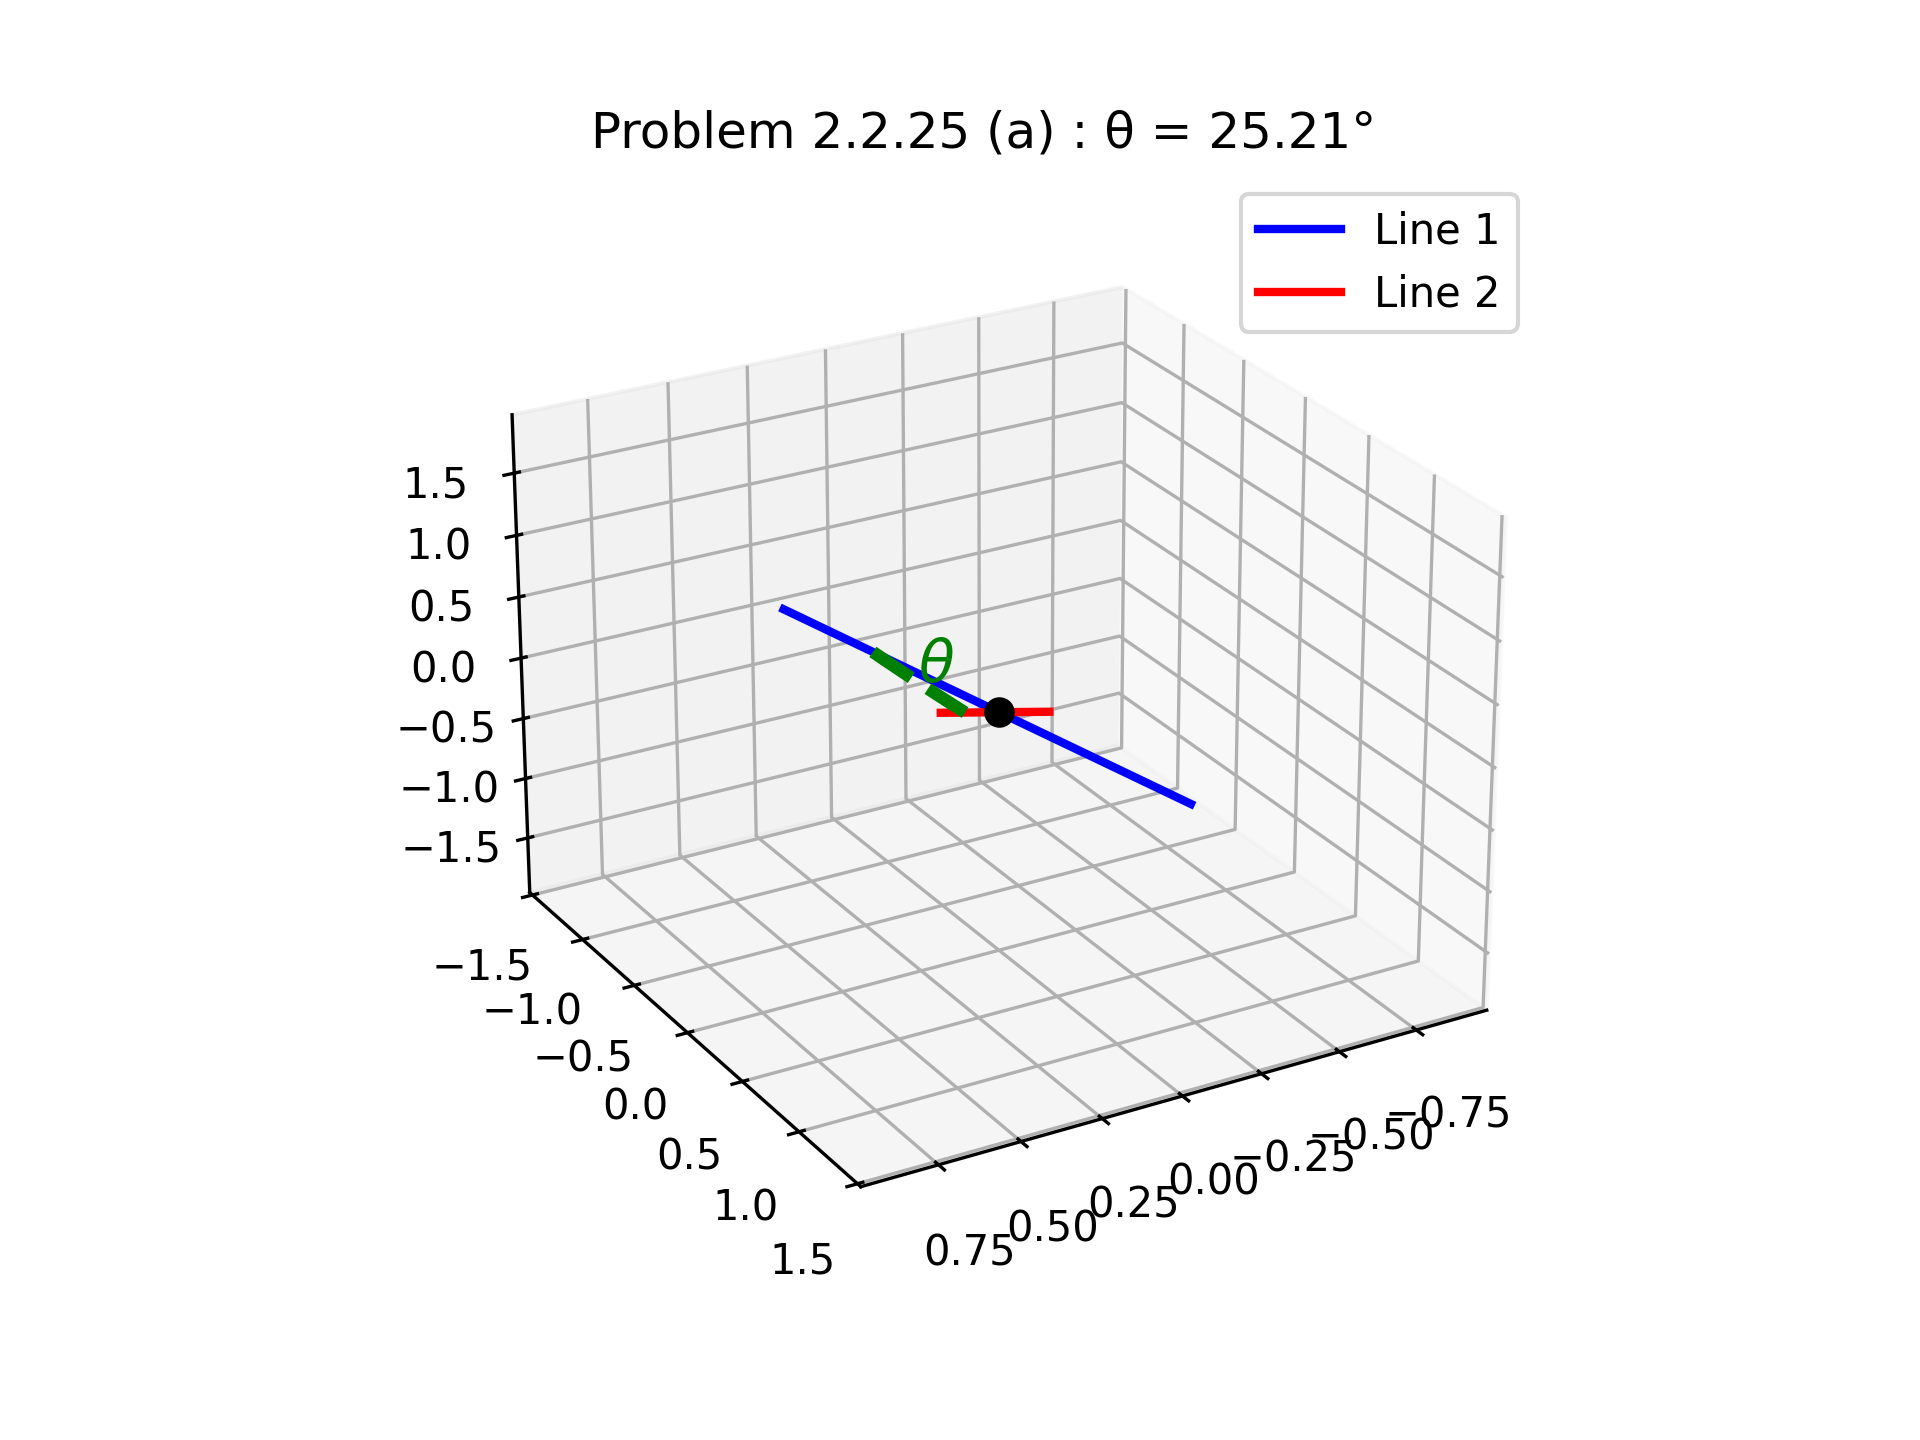
\includegraphics[width=1\columnwidth]{figs/figure_a.png}
    \caption{}
    \label{fig:placeholder}
\end{figure}

\begin{figure}[H]
    \centering
    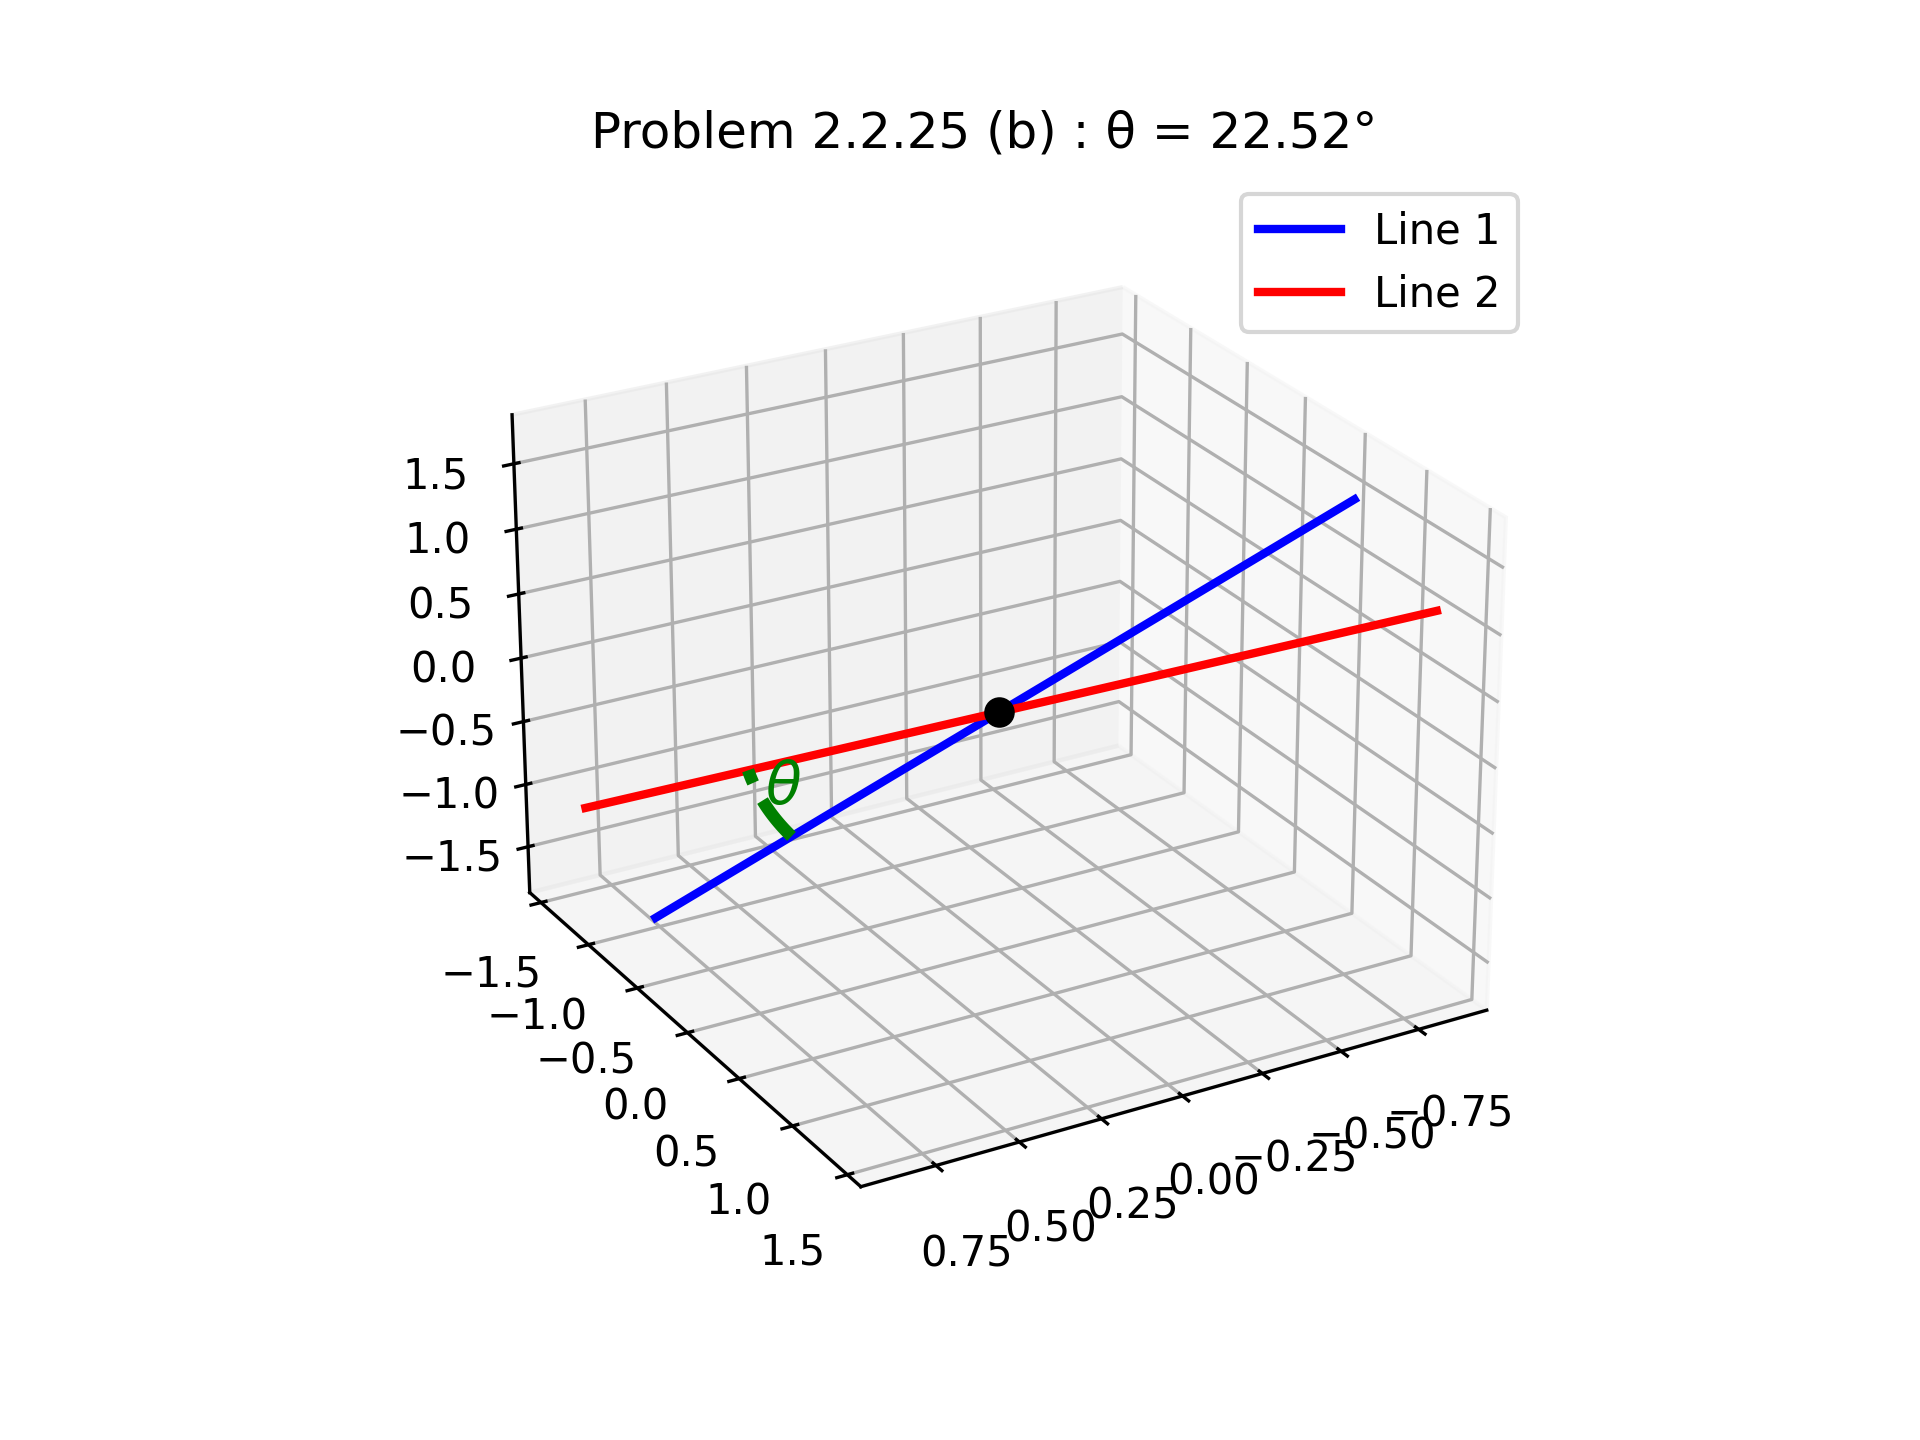
\includegraphics[width=1\columnwidth]{figs/figure_b.png}
    \caption{}
    \label{fig:placeholder}
\end{figure}

\begin{figure}[H]
    \centering
    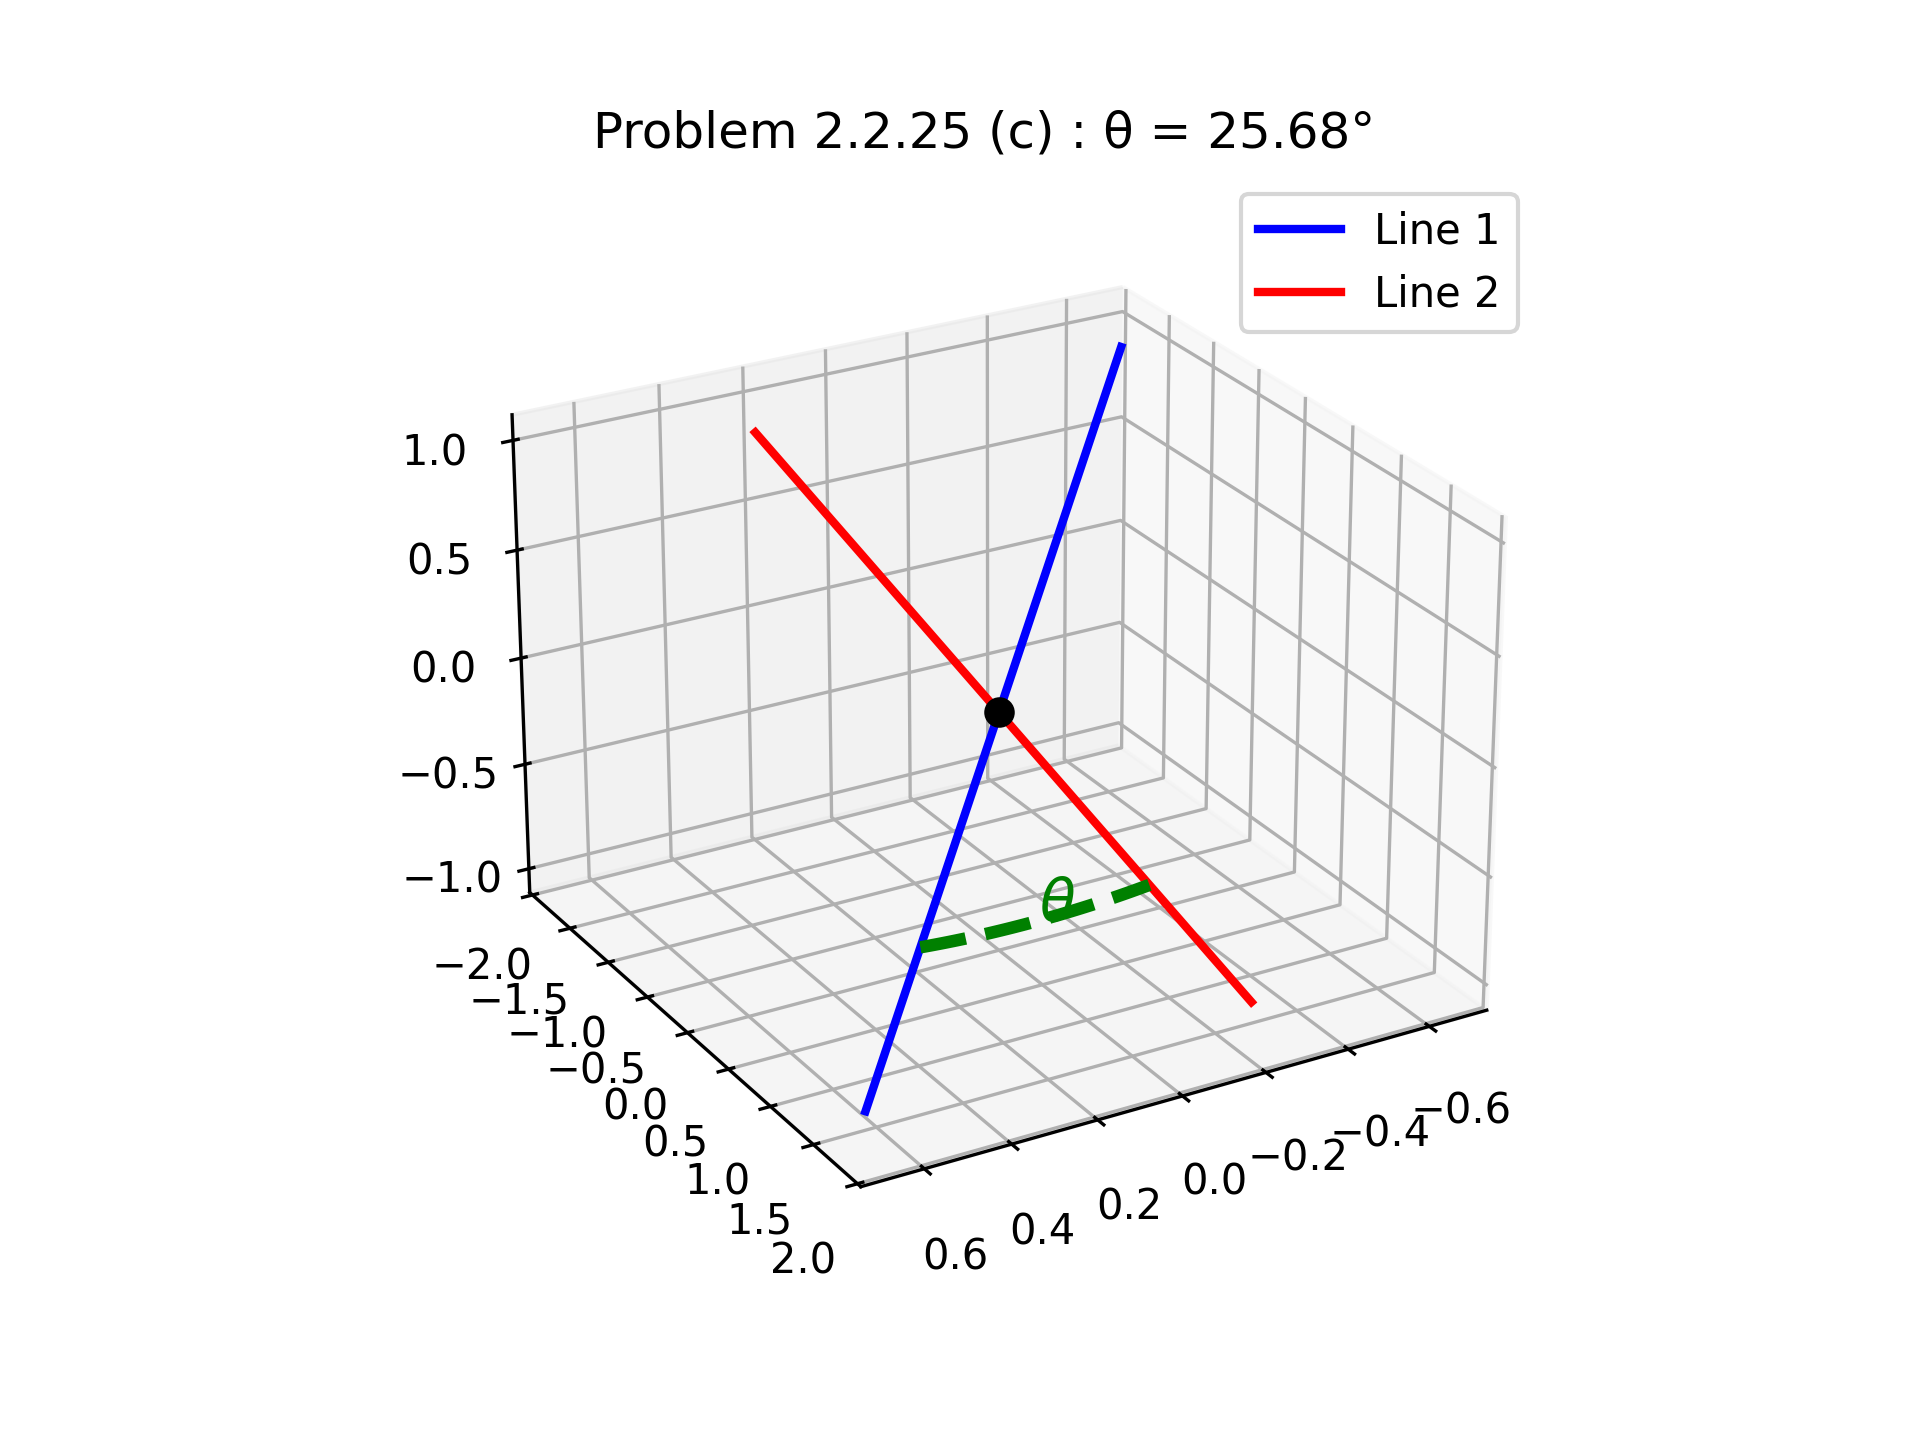
\includegraphics[width=1\columnwidth]{figs/figure_c.png}
    \caption{}
    \label{fig:placeholder}
\end{figure}

\begin{figure}[H]
    \centering
    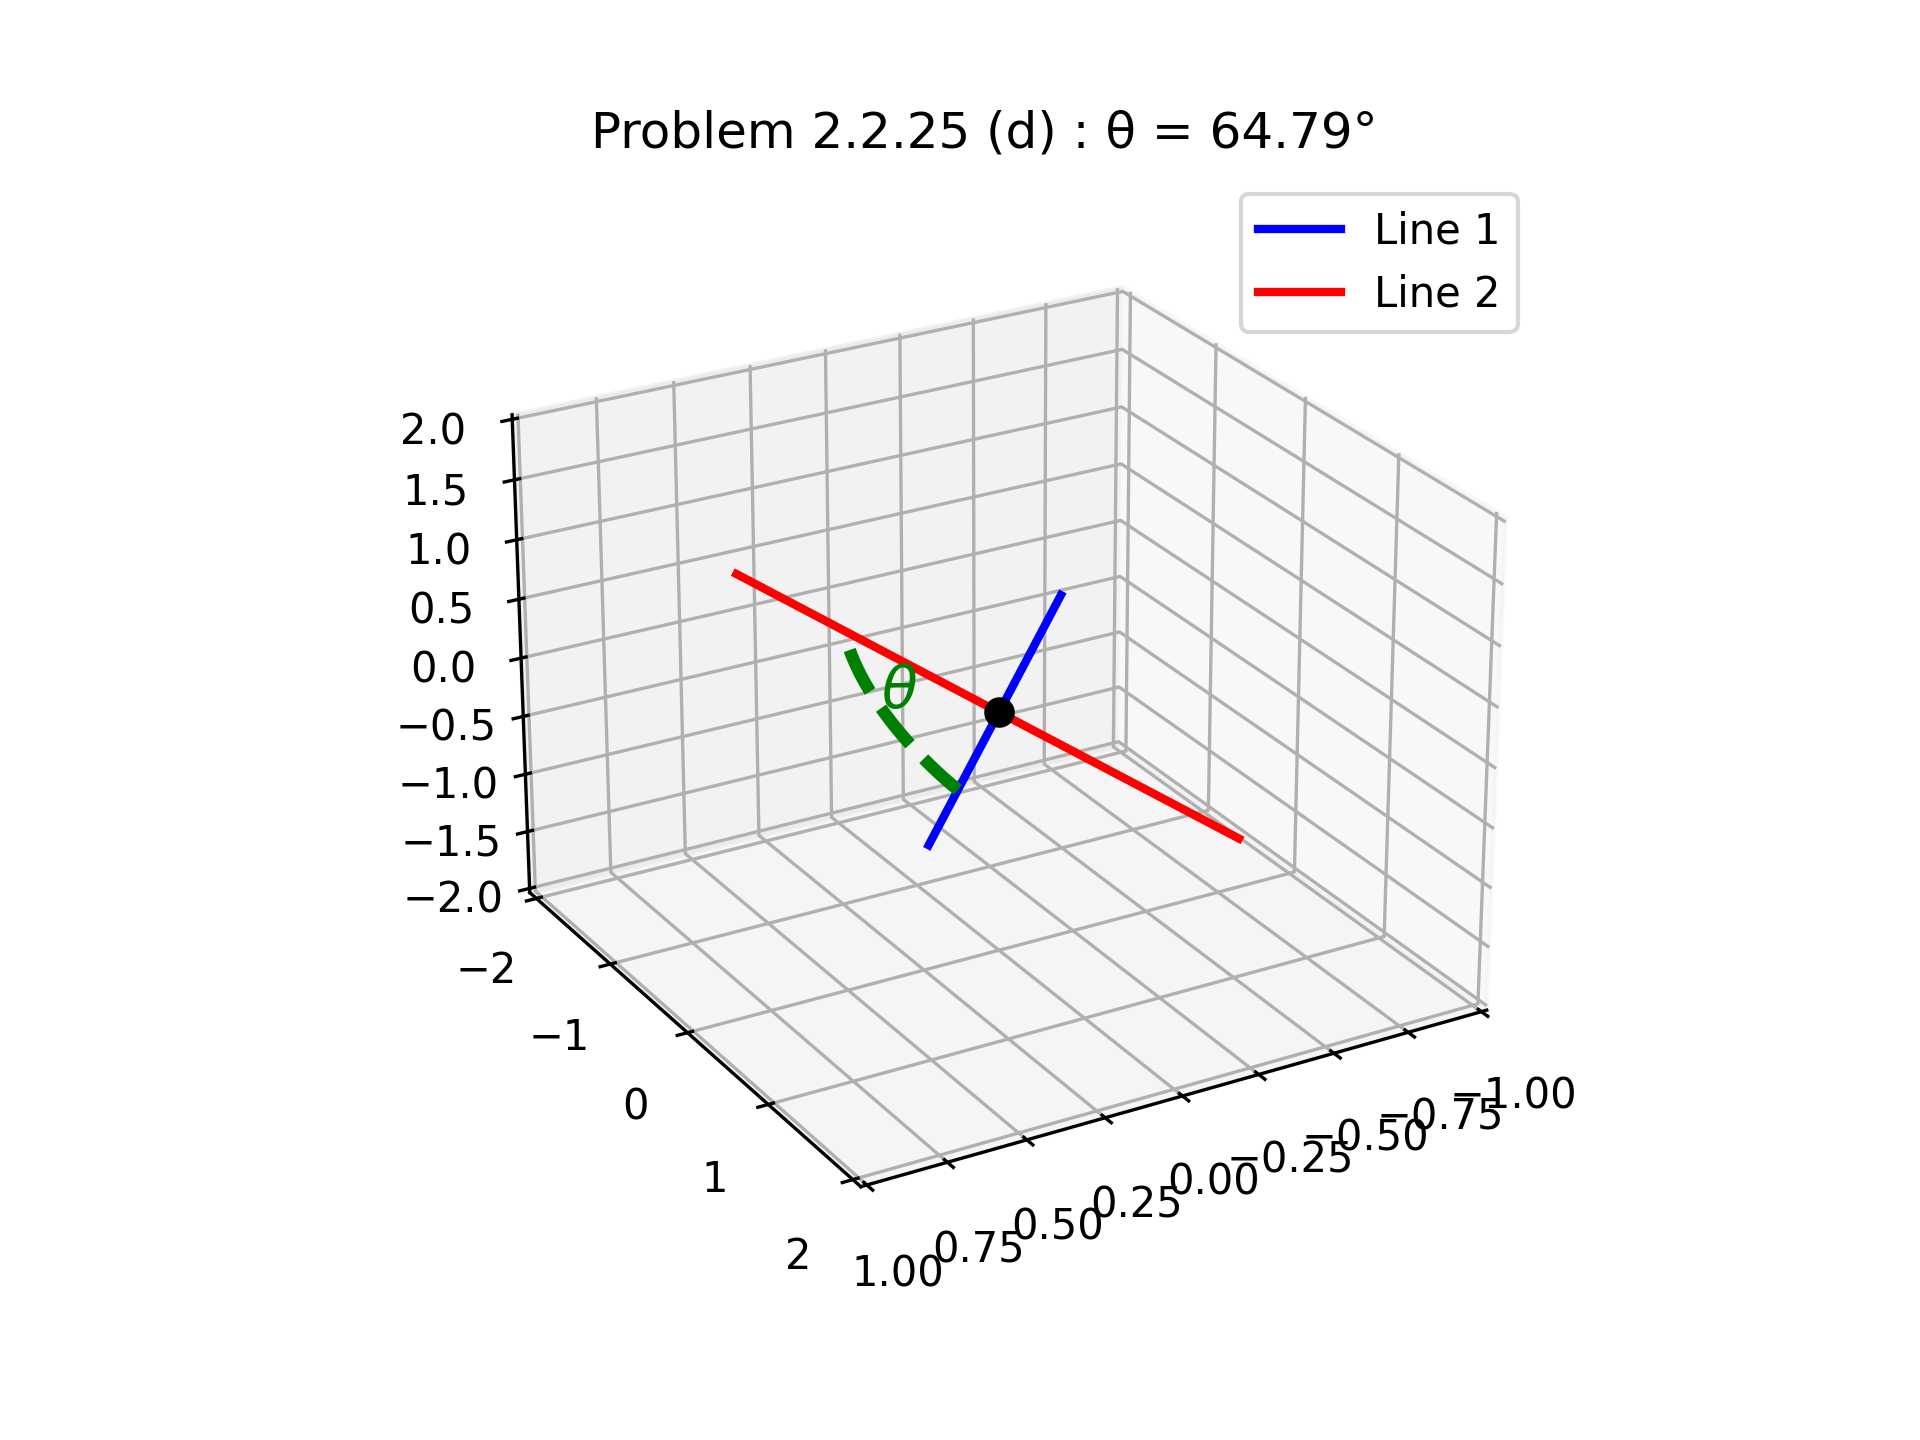
\includegraphics[width=1\columnwidth]{figs/figure_d.png}
    \caption{}
    \label{fig:placeholder}
\end{figure}

\end{multicols}

\end{document}
